\item {\bf Programming assignment}

In this programming assignment, we will use an autoregressive generative model to create text. We will 
generate samples from the recent \href{https://openai.com/research/better-language-models}{OpenAI GPT-2 model}. 
It is a model based on the Transformer, which is a  special kind of autoregressive model built on self-attention blocks, and 
has become the backbone of many recent state-of-the-art sequence models in Natural Language Processing. 
See this \href{https://jalammar.github.io/illustrated-transformer/}{blog} post for a friendly introduction. You will be asked to implement the sampling procedure for this model and compute likelihoods. 

In Figure \ref{fig:gpt}, we show an illustration on how this model (roughly) works. Consider a sequence of tokens $x_0,x_1,...,x_T$. 
For each token $x_i$, it has 50257 possible values. First, for each possible value of a token, we use a 768-dimensional 
trainable vector as its embedding, which results in a total of 50257 different embedding vectors. Next, we feed 
the embeddings into a GPT-2 network. The output vectors of the GPT-2 network are finally passed through a fully-connected 
layer to form a 50257-way softmax representing the probability distribution of the next token $p_{i+1}$. See Figure \ref{fig:gpt} for an illustration.

Training such models can be computationally expensive, requiring specialized GPU hardware. In this particular assignment, 
we provide a smaller pretrained model. It should be feasible to run this model without using any GPUs. 
After loading this pretrained model into \texttt{PyTorch}, you are expected to implement and answer the following questions.

\begin{figure}[h]
    \centering
    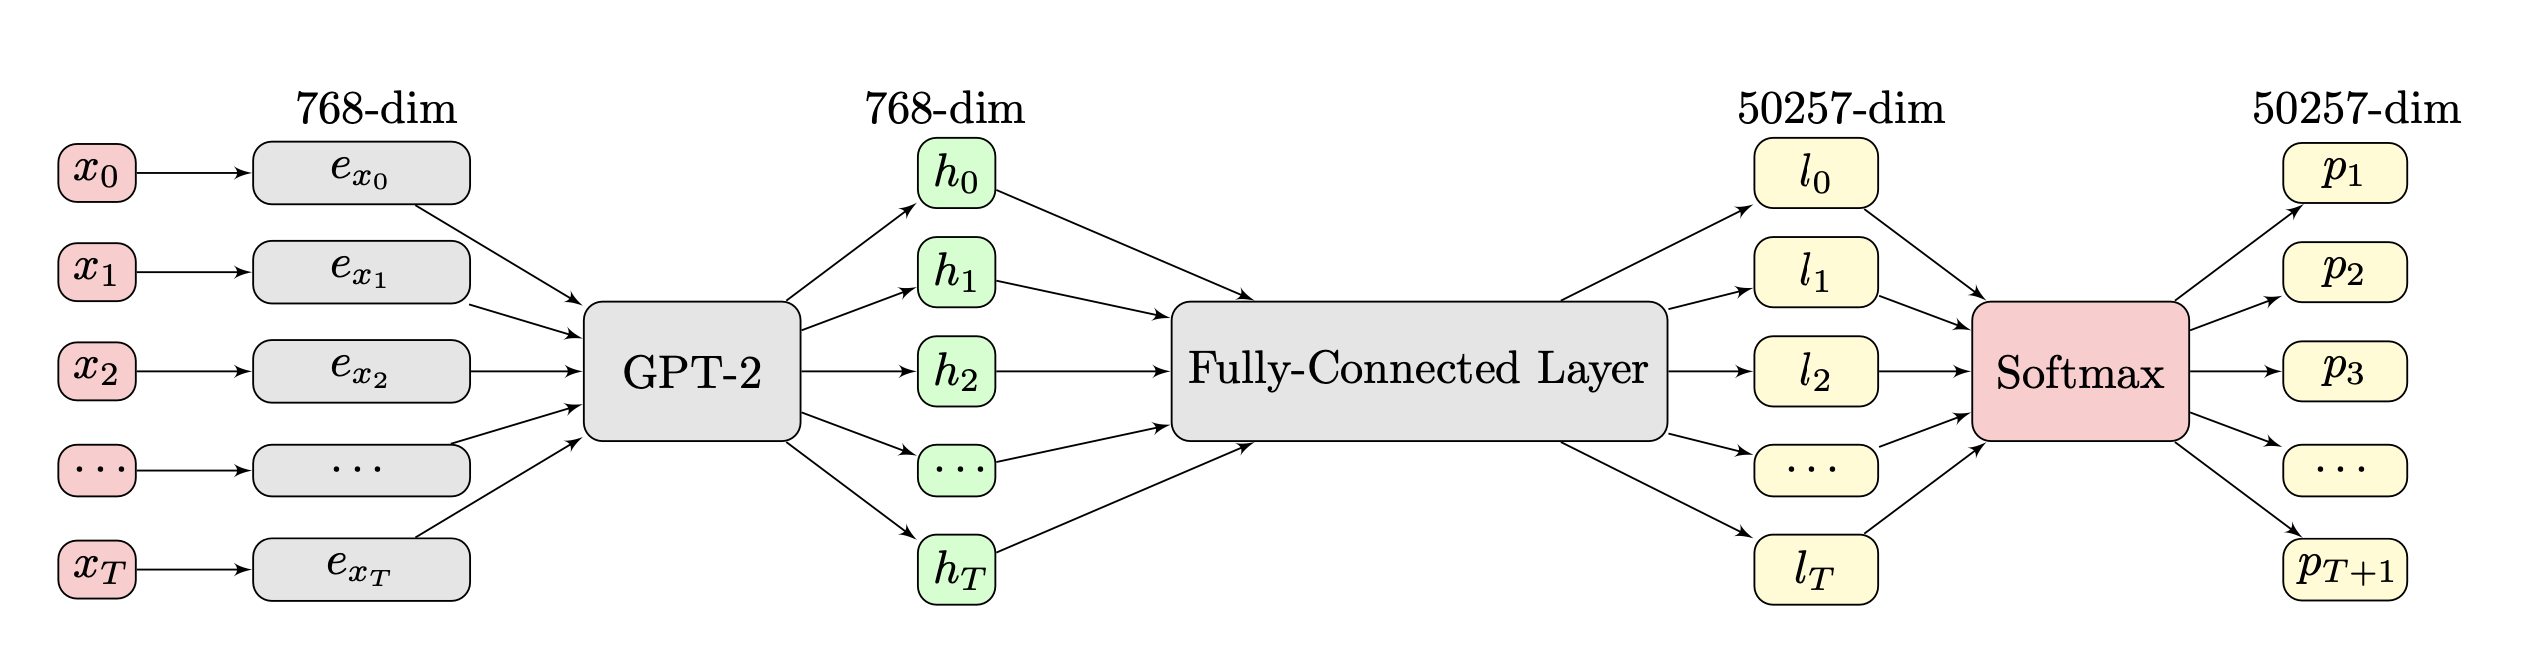
\includegraphics[width=0.9\textwidth]{./figures/gpt-2}
    \caption{The architecture of our model. $T$ is the sequence length of a given input. $x_i$ is the index token. $e_{x_{i}}$ is the trainable embedding of token $x_i$. $h_i$ is the output of GPT-2. $l_i$ is the logit and $p_i$ is the probability. Nodes in gray contain trainable parameters.}
    \label{fig:gpt}
\end{figure}

To run the models for 6.c through 6.f, please run
\begin{verbatim}
  python main.py 
\end{verbatim}

For GPU acceleration run run the command below. \textbf{Note:} we are not supporting MPS GPUs as it trains slower than CPU-enabled training on Apple Silicon devices. 
\begin{verbatim}
  python main.py --device gpu
\end{verbatim}

\begin{enumerate}

  \input{06-code/01-bit}

  \input{06-code/02-params}

  \item \points{6c}

In this question, we will try to generate paper abstracts using the GPT-2 model. We will first implement the sampling
procedure for GPT-2. Then, we will choose 5 sentences from the abstracts of some NeurIPS\footnote{Neural Information Processing Systems (NeurIPS) is a machine learning conference.} 2015 papers and see how GPT-2 generates the 
rest of the abstract. You will need to complete the method sample in \texttt{src/submission/sample.py} in the starter code.

\textbf{Hint}: The text generated should look like a technical paper.

  \item \points{6d}

Complete the function \texttt{log\_likelihood} in \texttt{src/submission/likelihood.py} to compute the log-likelihoods for each string. 
The histograms of the log-likelihoods of strings for each file should look like those in Fig. \ref{fig:ll}.

\begin{figure}
    \centering
    \begin{subfigure}{0.3\textwidth}
        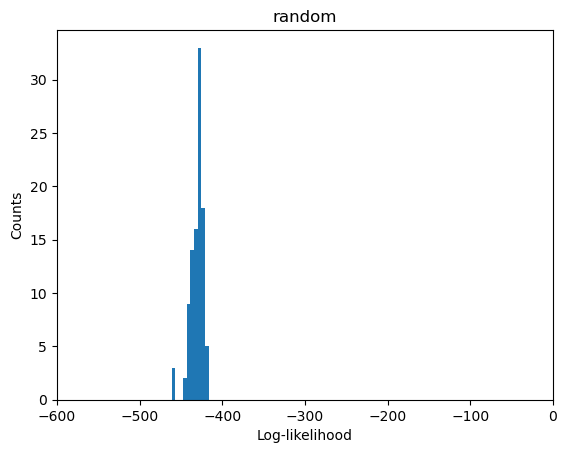
\includegraphics[width=\linewidth]{./figures/random}
    \end{subfigure}
    \begin{subfigure}{0.3\textwidth}
        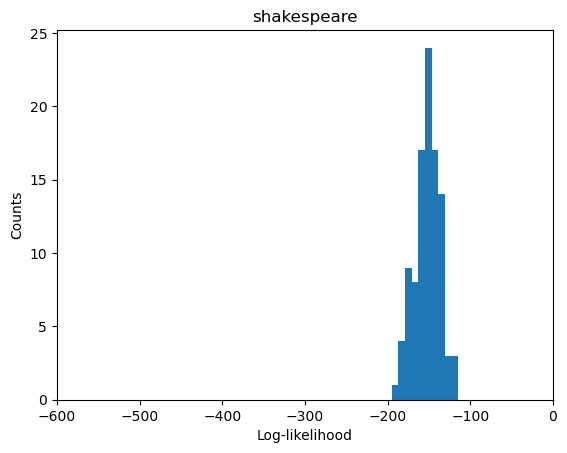
\includegraphics[width=\linewidth]{./figures/shakespeare}
    \end{subfigure}
    \begin{subfigure}{0.3\textwidth}
        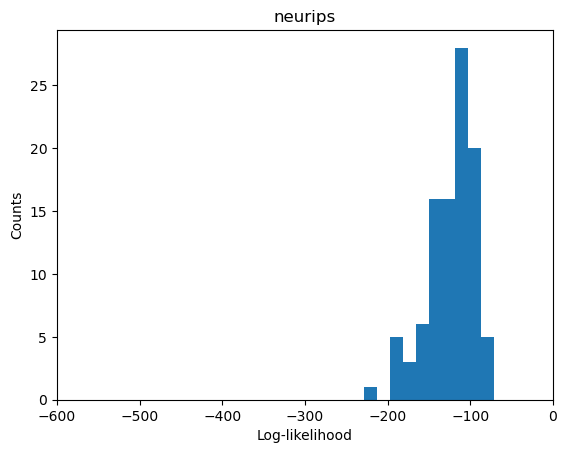
\includegraphics[width=\linewidth]{./figures/neurips}
    \end{subfigure}
    \caption{Expected log likelihood histograms for each text type}
    \label{fig:ll}
\end{figure}

  \item \points{6e}

We now provide new texts in \texttt{snippets.pkl}. The texts are either taken from NeurIPS 2015 papers or Shakespeare’s work, 
or generated randomly. Try to infer \textbf{whether the text is random}. You will need to complete the function \texttt{classification} in 
\texttt{src/submission/classifier.py}.

\textbf{Hint}: Look carefully at the plots above in Fig. \ref{fig:ll}. Is there a simple representation space in which the 
random data is separable from the non-random data?



  \item \points{6f}

Temperature scaling is a commonly used technique for adjusting the likelihood of the next token. We pick a scalar temperature
$T > 0$ and divide the next token logits by $T$:

\begin{equation} \label{eq:14}
    p_{T}(x_i \mid x_{<i}) \propto e^{\log p(x_i \mid x_{<i})/T}
\end{equation}


The model $p$ is the GPT-2 model used in question (6.c) and the model $p_T$ is the temperature-scaled model. For $T < 1$, 
we can see that $p_T$ induces a \textit{sharper} distribution than $p$, since it makes likely tokens even more likely.

Complete the function \texttt{temperature\_scale} in \texttt{src/submission/sample.py} only for 

the case when \texttt{temperature\_horizon=1} 
to perform temperature scaling during sampling.

  \input{06-code/07-joint-temp}

  \item \points{6h}

Next, we will implement temperature scaling over more than than one token (for simplicity, we will do
temperature scaling over two tokens).

\begin{equation} \label{eq:17}
    p_{T}^{\texttt{joint-2}} (x_i, x_{i+1} \mid x_{<i}) \propto e^{\log p(x_i,x_{i+1} \mid x_{<i})/T} \\
\end{equation}

\begin{equation} \label{eq:18}
    p_{T}^{\texttt{joint-2}} (x_i \mid x_{<i}) = \sum_{j} p_{T}^{\text{joint-2}} (x_i, x_{i+1} = a_j \mid x_{<i})
\end{equation}

Complete the function \texttt{temperature\_scale} in \texttt{src/submission/sample.py} for the 

case when \texttt{temperature\_horizon=2} 
to perform temperature scaling over a horizon of two tokens.


\end{enumerate}

